\section{Calibration Production and Application} \label{sec:calibration-production}
% former label: sec:processing:calibration

Some artifacts removed in the ISR sequence described in \S\ref{sec:isr-science} require a calibration data product that characterizes the instrumental effect being removed, measured in advance from dedicated calibration exposures rather than from the science image itself.
In this section, we describe in detail the algorithms used to produce calibrations and apply them to an image in ISR.
Figure~\ref{fig:calib-dependency} summarizes calibration-product dependencies.

\begin{figure}[t!]
    \centering
    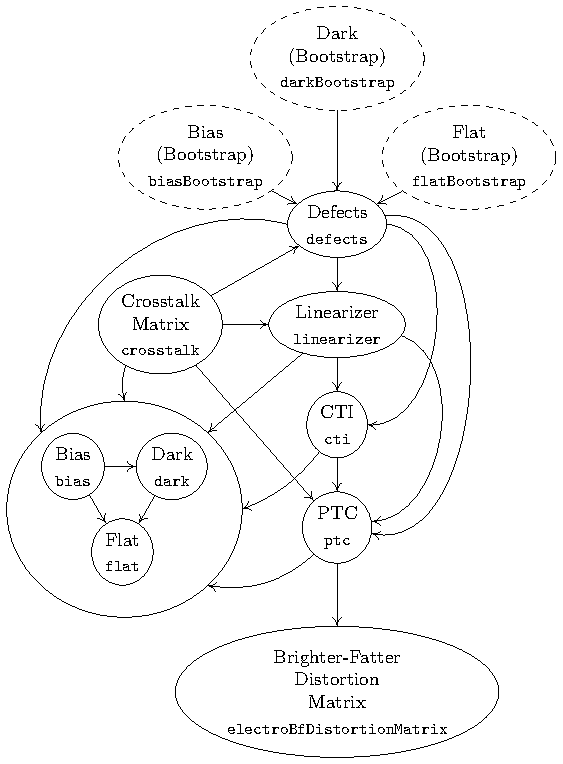
\includegraphics[width=\columnwidth]{figures/calib-dependency.pdf}
    \caption{Calibration production dependency graph.
    Arrows indicate data or dependency flow (``x $\rightarrow$ y'' means ``y depends on x'').
    Solid outlined boxes represent datasets that are deployed/released with data products while dashed boxes represent internal or intermediate datasets that are not formally released to users.}
    \label{fig:calib-dependency}
\end{figure}

% NOTE: order follows calib-dependency figure

\subsection{Curated Calibrations} \label{sec:processing:calibration:curated-calibs}

\subsection{Auxiliary Data Products} \label{sec:processing:calibration:auxiliary-data-products}

\subsection{Crosstalk} \label{sec:processing:calibration:xtalk}
Large astronomical sensors are read out through multiple amplifiers in parallel (see Section \ref{sec:lsstcam}), reducing the time needed to completely read the sensor.
One downside of this design strategy is the possibility of inducing crosstalk between the different amplifier channels.
In LSSTCam, this crosstalk is produced by electronic coupling that occurs in at least two different places in the readout hardware: (1) between the channels in the cable connecting the detectors to the REB and (2) across opposite sides of each detector with neighboring analog signal-processing integrated circuits (ASPICs). 
The result of these couplings is that the data for a particular amplifier shows a scaled copy of neighboring amplifiers added to the image.\todo{Give the typical and maximum crosstalk coefficient magnitudes measured for LSSTCam (e.g.\ $\sim10^{-4}$ nearest-neighbour, $<10^{-5}$ elsewhere), and how the two coupling mechanisms differ in strength.}
As all amplifiers are clocked through the readout process simultaneously, this scaled copy is aligned with the location of the readout corners.
This may make the crosstalk signal visible in the target amplifier flipped relative to the source amplifier.
These two sources cannot be disentangled from one another, so we measure and correct both forms of crosstalk as a single artifact.

Correcting for this additional signal is easy with a known set of crosstalk coefficients between a given source and target amplifier. Each source amplifier that has a non-zero coefficient is flipped to match the target amplifier, scaled by that coefficient, and added to the results from all other source amplifiers to create a subtrahend image that contains all of the crosstalk signal observed on the target amplifier.
By repeating this for all amplifiers, we can build up a full-detector subtrahend image that can then be subtracted.
As this correction may be imperfect, we set a CROSSTALK mask plane for all locations where the subtrahend image is greater than 1 electron.\todo{Quantify ``may be imperfect'': the residual crosstalk after correction (as a fraction of the uncorrected signal, cf.\ Figure~\ref{fig:crosstalk-linear-nonlinear-fit}) and the typical fraction of pixels flagged CROSSTALK in a science image.}
This provides a way for the downstream object detection and measurement code to identify sources that may have been significantly altered by the crosstalk correction.

As this crosstalk occurs in the cable connecting the detector to the REB, prior to being digitized into ADU, the images need to be gain corrected prior to the crosstalk correction to ensure they are in electron units.
This naturally places the crosstalk correction early in the ISR processing. This is also important because very bright sources can create bleed trails that deposit charge that is not fully clocked out, and that slowly leaks out as subsequent rows are read out.
These bleed trails can extend into the parallel overscan region, which can in turn create crosstalk signal in neighboring amplifiers.
Performing crosstalk correction prior to overscan correction prevents these amplifiers from oversubtracting the affected columns.

The crosstalk coefficients used during commissioning were calibrated from lab measurements at SLAC prior to the camera being shipped to the summit and were quadratic with the source flux, as discussed in \citet{2021JATIS...7d48002S} (CZW: do we need to introduce the measurement process first?).
However, the switch from 2s readouts to 3s readouts via a camera sequencer change invalidated these coefficients, as the change in clocking also changed the scale of the crosstalk signal, requiring this calibration to be remeasured.\todo{State by how much the coefficients changed between the 2\,s and 3\,s sequencers (a typical ratio or percent shift), which is what justifies the remeasurement.}

This measurement used three nights (CZW: check numbers in this paragraph) of spot data taken with the CBP system.
Each exposure placed one spot on each detector, with ten linearly spaced flux levels (CZW: add figure or describe levels) per pointing.
After the flux sequence was completed, the CBP spots were shifted to land on a different amplifier, with the process repeated in order to provide each amplifier a bright source to use to look for crosstalk signals.
A total of XX exposures were used to generate these updated crosstalk coefficients, with the number of pixels used as ``source pixels'' (CZW: which you haven't explained yet) shown in Figure~\ref{fig:crosstalk-source-pixels}.

\begin{figure}[t]
    \centering
    % TODO: add exposure-time vs.\ mean-signal figure asset
    \fbox{\parbox{0.75\columnwidth}{\centering\vspace{1.5in}\small\textit{Figure pending}\vspace{1.5in}}}
    \caption{Number of source pixels used to measure the crosstalk coefficients for each amplifier.
      Note that this number drops toward the edge of the focal plane, due to difficulties properly illuminating CBP spots in these locations.\todo{Quantify the drop-off: typical source-pixel counts at the focal-plane centre vs.\ the edge, and the minimum count below which a coefficient was considered unconstrained.}}
    \label{fig:crosstalk-source-pixels}
\end{figure}

As discussed above (CZW: ???), each of these exposures was minimally processed to correct the serial overscan, apply the gains to convert the units to electrons, and to trim and assemble the data segments.
All pixels above a threshold of 30,000 electrons were then identified and used to construct crosstalk ratios $r_{ij} = T(\hat(x), \hat(y))_j / S(x, y)_i$, where $S(x, y)_i$ is the flux value in a pixel at $(x, y)$ in amplifier $i$, and $T(\hat(x), \hat(y))_j$ is the flux value at the same ``readout coordinate'' $(\hat(x), \hat(y))$ in amplifier $j \ne i$.
These ratios therefore show the measured response to the source signal $S$ at the expected location of a crosstalk source at a target location $T$.
These fluxes and ratios are accumulated for the entire set of exposures and detectors.
Prior to any further study, the ratios are clipped to ensure contaminating features, such as stray light and reflections of other spots, are removed.\todo{Report what fraction of ratio measurements the clipping removes, so the reader can judge how aggressive the cleaning is.}
Any pixel with a measured ratio larger than 1.0 are excluded, as these would represent an unphysical situation in which the crosstalk signal was brighter than the source signal.
The remaining signals were XX-sigma clipped based on the inter-quartile distance, under the assumption that the ratio values are normally distributed.

If the crosstalk response was perfectly linear, the average of these clipped ratios would directly yield the crosstalk coefficient between the source and target amplifiers.
However, as shown in the lab study of the crosstalk, and demonstrated in Figure~\ref{fig:crosstalk-linear-nonlinear-fit}, such a simple model fails to fully remove the crosstalk, as the source brightness changes over the profile of the spot.\todo{Quantify the improvement from the non-linear model: residual amplitude (in electrons or as a fraction of source flux) for the linear vs.\ non-linear coefficients shown in the two panels of the figure.}

\begin{figure}[t]
    \centering
    % TODO: add exposure-time vs.\ mean-signal figure asset
    \fbox{\parbox{0.75\columnwidth}{\centering\vspace{1.5in}\small\textit{Figure pending}\vspace{1.5in}}}
    \caption{An example crosstalk residual on LSSTCam detector XX after correction with a linear crosstalk coefficient.
      The oversubtraction in the core and undersubtraction in the wings of the source illustrates that the strength of the crosstalk signal is dependent on the flux of the source pixel.
      The right panel shows the same spot, as corrected with the final non-linear crosstalk coefficients.}
    \label{fig:crosstalk-linear-nonlinear-fit}
\end{figure}

To provide the required crosstalk coefficients that are non-linear in source flux, we quantified the evolution of crosstalk coefficients with a linear term and a non-linear term in the fit to the flux ratios.
The intercept of this fit provides the term that is linear in the source flux, and the slope of the fit provides a term quadratic in the source flux.

\subsection{Defects} \label{sec:processing:calibration:defects}

We build a \textsc{defects} calibration product based on defects manually defined and automatically detected.
They correspond to pixels whose output is not well corrected by our ISR approach.\todo{Quantify the defect population for DP2: total number of masked pixels/columns, the fraction of the focal plane they represent, the split between manual and automatic detections, and how that fraction varies between E2V and ITL and across epochs.}
These defect pixels are masked and marked as \textsc{BAD} for the downstream analysis and interpolated over for visual inspection.

The \textsc{defects} calibration product is constructed by measuring defects on bias, dark, flats and then merged together.
The defect detection consists of the following steps:
\begin{itemize}
    \item correct for the gradient across the focal plane, by applying a gradient correction to each amplifier
    from the gradient measured in a binned image.
    \item a background estimate is done and removed,
    \item hot pixels are defined as bright pixels with more than 5~electrons/s (scaled by the exposure time) of dark current, above 1000 ADU in bias are measured,
    \item cold pixels are defined as pixels with photoresponse less than $80\%$ of the flat mean are measured,
    \item pixels along the midline break (the interface between the top and bottom amplifiers) in E2V detectors are
    set to the median of the flats (so they are not found by the defect code),
    \item bad columns masking.
\end{itemize}

Afterwards, these measured defects are merged together, and the edges of the detectors are masked, to
mask what we refer to as the ``picture frame'' effect corresponding to the presence of distorted electric fields at the edges of the CCDs.\todo{Give the edge-mask width in pixels and the measured size of the ``picture frame'' response distortion (percent deviation from the detector interior) that motivates that width.}

For DP2, these defects were produced by using ``bootstrap'' versions of the bias, dark, and flat, as these calibration products need the defects themselves to be defined.
This will probably be updated in future iteration of calibration products.

Additionally manual defects are large features present in LSSTCam detectors, such as the large defect in detector 0
which induces large bleeds.\todo{Quantify ``large'': the size of the detector 0 defect and the typical extent of the bleeds it induces, plus how many detectors carry manual defects of this scale.} LSSTCam manual defects are defined in \url{https://github.com/lsst/obs_lsst_data/tree/main/lsstCam/manual_defects}.
%We describe how defect masks are generated (bad pixels/columns, saturation trails, and other artifacts), the thresholds used, and how masks are combined across exposures.

Further defect statistical analyses, description of the defect monitoring, masking optimization are postponed to a future paper.
Additional masking is applied to an exposure in the ISR processing, as described in Sec ??.
% TODO(ref): literal "Sec ??" -- point this at the ISR masking steps in \S\ref{sec:isr-science}.

\subsection{Non-Linearity} \label{sec:processing:calibration:linearity}

Non-linearity (NL) describes a deviation from simple proportionality when mapping amplified voltage integrated during readout to the number of analog-to-digital units (ADU) or counts.
Non-linearity is signal-dependent and is often not a simple function of signal level; it can change suddenly above a large signal level that is characteristic to each readout amplifier; and it can drift with sensor temperature and with time, as slow electronic shifts in the bias level accumulate over a long calibration campaign.\todo{Quantify the drifts: the fitted $\alpha$ (per K) and $\beta$ (per day) sensitivities and the resulting non-linearity change over a typical campaign, plus the range of per-amplifier turnoff levels implied by ``characteristic to each readout amplifier''.}
In practice it introduces pixel-level measurement bias (up to x\% from the true signal) and invalidates Poisson counting statistics and can interfere with measurement of gain (which shouldn't change or drift with signal level).\todo{Fill in $x$ with the measured uncorrected non-linearity amplitude, and say over what signal range it applies.}
Correcting NL to better than y\% is therefore a prerequisite for reliable downstream calibration products and science analyses.\todo{Fill in $y$ with the requirement, cite its source, and state the residual level actually achieved by the double-spline model for DP2.}

We can measure non-linearity by measuring the response of pixel values to a change in illumination level.
The in-dome calibration illumination system can deliver an approximately uniform flux of light across the LSSTCam focal plane.\todo{Say how uniform ``approximately uniform'' is (percent variation across the focal plane), since the relative-spline step exists specifically to absorb this non-uniformity.}
Given a known change in some input illumination level, we should be able predict a change in the number of counts in an image, which we can then compare to the measured change counts.

We have independent measurements of the photodiode current produced by our calibration illumination system that we can integrate with the exposure time and use as a baseline truth of the amount of incident light while taking an exposure,
however we found these measurements to be noisy and unreliable.\todo{Quantify ``noisy and unreliable'': the fractional scatter of the integrated photodiode current relative to exposure time, compared with the shutter-timing accuracy, to justify the substitution.} Instead we use the exposure time, which is precisely measured and makes a natural proxy for photodiode measurements.
We therefore calibrate NL by fitting a relation between exposure time ($\Delta t$, abscissa) and the mean measured flat-field signal ($\mu$, ordinate).

We measured $543\times2$ flat-field exposures at evenly spaced illumination levels. We went as low as 100~analog-to-digital units (ADU) and continued beyond pixel saturation.\todo{State the amplitude and signal range of the observed low-signal non-linearity below this 100~ADU floor (percent deviation below what ADU level), so the disconnected box in Figure~\ref{fig:detector-boxes} and the missing DNL correction flagged in \S\ref{sec:limitations} are backed by a number.}
At each illumination level, a pair of flats was acquired by varying both LED current and exposure time to achieve the targeted levels, measuring the mean signal level as $\mu_i = \mathrm{avg}(F_i^{(1)},F_i^{(2)})$~(in ADU).
These data were acquired with illumination levels decided in random order to decouple signal-dependent non-linearity and time-dependent drifts in illumination.

\begin{figure}[t]
    \centering
    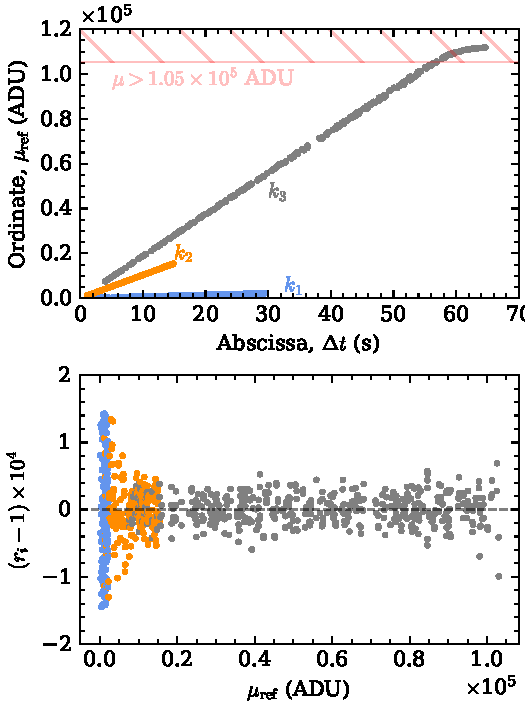
\includegraphics[width=0.95\columnwidth]{figures/reference-amp-non-linearity_det94.pdf}
    \caption{Absolute non-linearity fit for the reference amplifier~C07 on LSSTCam detector~94.
    \textit{Left}---mean flat-field signal $\mu_{\mathrm{ref}}$ as a function of exposure time $\Delta t$, colored by LED illumination group ($k_1$, $k_2$, $k_3$).
    Each group has its own ratio of signal to exposure time, which produces the discontinuities between groups.
    The hatched region marks signal above the linearity turnoff ($\mu > 1.05 \times 10^5$~ADU), which is excluded from the fit.
    \textit{Right}---fractional residuals of the spline fit, $(r_i - 1) \times 10^4$ (Equation~\ref{eq:spline-nl-fit}), as a function of $\mu_{\mathrm{ref}}$, with the same group colors.}
    \label{fig:linearity-exptime-vs-signal}
\end{figure}

Figure~\ref{fig:linearity-exptime-vs-signal} shows the resulting relation for a representative amplifier.
Discontinuities appear at the boundaries between LED current settings, producing different signal levels for the same exposure time.
These data are partitioned into groups associated with distinct LED illumination settings.
Grouping is determined either from exposure metadata or by computationally searching for jumps in the ratio of mean detector signal to exposure time.
Within each group we allow a distinct proportionality constant $k_j$ to capture the size of the jumps.

To first order, the trend between exposure time and the mean measured flat-field signal over properly scaled groups is linear and related to the intrinsic gain in each readout channel.
We can fit a simple slope and intercept to this trend to the low signal points; the highest signal level in each channel above which this approximation break is the ``linearity turnoff'' (as indicated in Figure~\ref{fig:linearity-exptime-vs-signal}).
Points above the turnoff are excluded from the NL fit because there is a maximum signal above which the measured counts can no longer be trusted due to hardware limitations at the output of the detector (Figure~\ref{fig:detector-boxes}).

\begin{figure}[t]
    \centering
    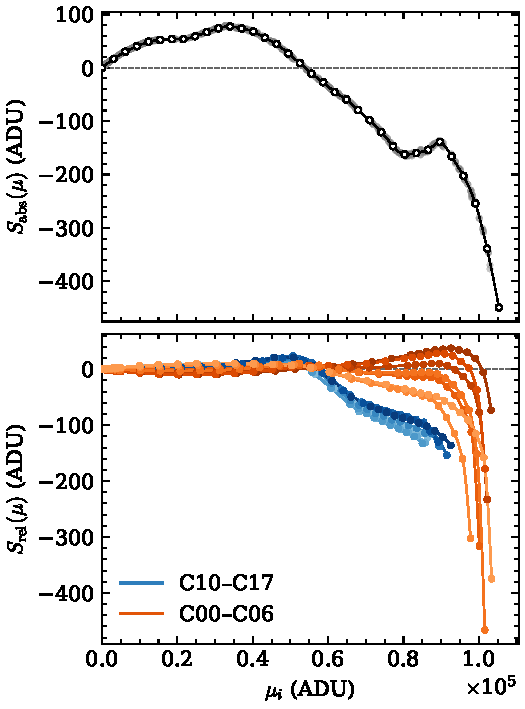
\includegraphics[width=0.95\columnwidth]{figures/abs-rel-non-linearity_det94.pdf}
    \caption{Double-spline non-linearity model for LSSTCam detector~94.
    \textit{Left}---absolute non-linearity $S_{\mathrm{abs}}(\mu)$ of the reference amplifier~C07.
    Gray points are per-exposure measurements (spline value plus fit residual), the black line is the Akima spline, and open circles mark the spline nodes.
    \textit{Right}---relative non-linearity $S_{\mathrm{rel}}(\mu)$ of the remaining amplifiers with respect to C07, with nodes shown as filled points.
    Blue shades are amplifiers C10--C17 and orange shades are C00--C06; darker shades correspond to higher segment numbers.}
    \label{fig:linearity-abs-rel}
\end{figure}

The NL model we fit to this relation is an extension of the formalism developed by \citet{2019A&A...629A..36A}.
We represent the deviation from linearity by an Akima spline $S(\mu)$ of the measured mean signal $\mu$.

For each exposure $i$ in group $j$ we define the residual ratio
\begin{equation}
    r_i = \frac{\mu_i - S(\mu_i) - O}{k_j\, D_{i}}
    \label{eq:spline-nl-fit}
\end{equation}
where $D_{i}$ is the data used for the abscissa (exposure time), $O$ is an optional constant offset that absorbs scattered light or other signal not proportional to $D_{i}$, and $w_i$ are weights.

The fit minimizes a uniformly weighted ($w_i = 1$) least-squares objective over all accepted points:
\begin{equation}
    \chi^2 = \sum_{i} w_i \left(r_i - 1\right)^2. \label{eq:linearity-chisq}
\end{equation}
The fit is subject to the boundary conditions $S(0) = 0$ and $\langle S(\mu)\rangle = 0$ over the fit range.
The first constraint fixes the origin such that zero illumination is always measured as zero signal; the second ensures that the spline captures deviations from linearity independently from knowing the true amplifier gain.

In addition, any hardware sensitivities are absorbed by nuisance parameters that we parameterize as first order linear corrections to $\mu$ before the spline is evaluated:
\begin{equation}
\begin{aligned}
    \mu &\rightarrow \mu \left(1 + \alpha\, T_i\right), \\
    \mu &\rightarrow \mu \left(1 + \beta\, t_i\right),
\end{aligned}
\label{eq:linearity-nuisance}
\end{equation}
where $T_i$ is a REB temperature (referenced to the median over the campaign), $t_i$ is the Modified Julian Date (MJD) of the midpoint of the shutter open time, and $\alpha$ and $\beta$ are fitted coefficients that describe each sensitivity.
For LSSTCam DP2 calibration production we fit only the temporal coefficients as well as the scattered-light offset $O$ on the spline.
For DP2, we found it to be unnecessary to fit the temperature coefficient since the temperature of the REB proved to be quite stable.\todo{Quantify ``quite stable'': the REB temperature range over the calibration campaign and the non-linearity error that neglecting $\alpha$ therefore incurs.}

We could perform this fit independently for every amplifier on every detector. However, most of the non-linearity is common to all amplifiers due to similar readout architectures, with only small amplifier-to-amplifier variations on top of that.\todo{Put numbers on ``most'' and ``small'': the amplitude of the absolute spline vs.\ the RMS of the relative splines (both readable off Figure~\ref{fig:linearity-abs-rel}), which is the quantitative justification for the double-spline decomposition.}
In addition, each independent fit to every amplifier would pick up not just the intrinsic non-linearity in amplifiers, but also exposure-to-exposure spatial illumination variation that occurs during the calibration campaign.
To better characterize this, it makes sense to perform a spline fit on each amplifier relative to both a single reference exposure and a reference amplifier on the same detector.

We can distinguish an \emph{absolute} non-linearity in a single reference amplifier on a detector and the \emph{relative} non-linearity of other amplifiers to that reference amplifier, the process for which is summarized in Algorithm~\ref{alg:linearity-double-spline} and illustrated in Figure~\ref{fig:linearity-abs-rel}.
After choosing a reference amplifier and a reference exposure, we do (1) a relative spline fit on every other amplifier using  the variation of its mean flat-field signal $\mu$ relative to the reference amplifier and to the $\mu$ in a single reference exposure, and then (2)
an absolute spline fit on the reference amplifier using the usual from $\mu$ versus $\Delta t$.
Every amplifier on a detector has a shared absolute spline fit based on the reference amplifier for that detector and a relative spline fit computed relative to a reference amplifier and a reference exposure ($S_{\mathrm{rel}}(\mu) = 0$ for the reference amplifier).

\begin{algorithm}[H]
\caption{Double-spline linearity fit (single detector)}
\label{alg:linearity-double-spline}
\begin{algorithmic}[1]
\For{each amplifier $a$}
    \State $k_j \leftarrow$ \Call{Find Groups}{$\mu_a$, $\Delta t$}
    \State \Call{Compute linearity turnoff}{$\mu_a$, $\Delta t$}
\EndFor
\State choose reference amplifier $\mathrm{ref}$ with the highest linearity turnoff
\State choose reference exposure $i_0$, the flat whose mean signal $\mu_{\mathrm{ref}} = 10^4$ on amplifier $\mathrm{ref}$ is nearest the target signal level
\For{each exposure $i$}
    % \State compare flat $i$ to the reference exposure $i_0$
    % \State $\mu_{\mathrm{ref},i} \leftarrow$  $\mu_{\mathrm{ref}}$ / $\mu_{\mathrm{ref}, i_0}$ % mean signal on amplifier $\mathrm{ref}$ in exposure $i$, normalized to $i_0$
    \For{each amplifier $a \neq \mathrm{ref}$}
        \State $D^{\mathrm{rel}}_{i} \leftarrow \mu_{\mathrm{ref}, i} \times (\mu_{a,i_0} / \mu_{\mathrm{ref}, i_0})$  (Relative Abscissa) % mean signal on amplifier $a$ in exposure $i$, normalized to $i_0$ and expressed relative to $\mu_{\mathrm{ref},i}$
        \State $\mu^{\mathrm{rel}}_{i} \leftarrow \mu_{a,i}$ (Relative Ordinate)
    \EndFor

    \State $D^{\mathrm{abs}}_{i} \leftarrow \Delta t_i$ (exposure time)
    \State $\mu^{\mathrm{abs}}_{i} \leftarrow \mu_{\mathrm{ref},i}$ (measured counts)
\EndFor

\Statex \Comment{Spline fit}
\State $S_{\mathrm{abs}}(\mu), O, \alpha, \beta \leftarrow$ \Call{Minimize}{Equation~\ref{eq:linearity-chisq}, $D^{\mathrm{abs}}_{i}$, $\mu^{\mathrm{abs}}_{i}$, $k_j$}
\State $S_{\mathrm{rel}}(\mu) \leftarrow$ \Call{Minimize}{Equation~\ref{eq:linearity-chisq}, $D^{\mathrm{rel}}_{i}$, $\mu^{\mathrm{rel}}_{i}$, $k_j$}
\end{algorithmic}
\end{algorithm}

To determine the corrected mean signal level, we can interpolate the Akima splines to compute a correction: $\mu' = \mu - S_{\mathrm{rel}}(\mu) - S_{\mathrm{abs}}(\mu)$.

If each amplifier is properly linearized around its true gain, we should observe in every exposure that the illumination level is coherent between amplifiers and detectors.
If the linearization is miscalibrated or biased (either because exposure time is not a good proxy for the true integrated photodiode or if constraining $\langle S(\mu)\rangle = 0$ is biased), the amplifiers and detectors will show signal-dependent fractional offsets in mean signal levels in each flat similar to a mis-estimation of gain.

We can check how the linearized mean signal levels deviate from an overall linear relation over some set of detectors in a given exposure:
For each exposure $i$, we form the linearized signal, $\mu'_i$, on the reference amplifier on every detector and compute the fractional residual:
\begin{equation}
    r_i = \frac{\mu'_i - m_i D_{i}}{y_i},
\end{equation}
where $m_i$ is the slope of a linear fit to $\mu'_i$ versus $D_{i}$.
We take the median $\langle r \rangle_i$ over a subset of focal-plane detectors (in the center of the focal plane) in that exposure and derive a multiplicative correction
\begin{equation}
    N_i = \frac{1}{1 - \langle r \rangle_i},
\end{equation} that we use to rescale the abscissa ($D_{i} \rightarrow N_i D_{i}$) and enforce that the linearization produces a coherent illumination across all detectors.

We can then re-compute the double-spline fit with the normalized abscissa on the reference amplifier. We can repeat the cycle (normalize, spline, normalize, etc.) recursively several times, each time computing the normalization as \begin{equation}
    N_i = \frac{N_i^{\mathrm{prev}}}{1 - \langle r \rangle_i}.
\end{equation}

A single iteration improves the precision of the linearity solution by a factor of \textcolor{red}{$N$}, with little further gain from additional iterations.\todo{Fill in $N$ and quantify ``little further gain'' --- e.g.\ the residual RMS after 1, 2, and 3 iterations --- and state how many iterations were used for DP2.} Because the normalization is derived from all the reference amplifiers, our measurement also benefits from the added statistical power which comes from combining measurements across the focal plane to calibrate each amplifier.\todo{Quantify the statistical gain from combining across the focal plane (number of reference amplifiers used and the resulting reduction in normalization uncertainty).}

In ISR, given an image with pixel values measured in counts ($F_{ij}$), the final spline model can be interpolated, providing a continuous map from measured counts to the corrected counts for any pixel value within the range of 0 signal to the linearity turnoff, computed as:
$F_{ij}' = F_{ij} - S_{\mathrm{rel}}(F_{ij}) - S_{\mathrm{abs}}(F_{ij})$.

% During science ISR, the linearizer is applied at the non-linearity correction step in Figure~\ref{fig:isr-pipeline}; see \S\ref{sec:isr-science}.


\subsection{Deferred Charge} \label{sec:processing:calibration:cti}

Several distinct effects in the readout chain displace charge from its pixel of origin and leave correlated structure in the serial overscan: (1) a pixel-to-pixel fractional loss during charge transfer referred to as ``global CTI'', (2) a local electronic-offset hysteresis in the output amplifier that mimics deferred charge in the first few overscan columns, and (3) localized capture and delayed release of charge by isolated trap sites in the serial register.
Strictly, only global CTI is ``charge transfer inefficiency'' in the textbook sense, but because all three enter at the same point in the photon transfer chain (Figure~\ref{fig:detector-boxes}) and produce overlapping signatures in the serial overscan, we model them together and produce a single calibration data product that we loosely refer to as ``CTI'' in Figure~\ref{fig:calib-dependency}.
These effects are measured, modeled, and corrected together using the extended pixel edge response (EPER) estimator developed for LSSTCam by \citet{2021JATIS...7d48002S}.

Calibrating deferred charge uses the same input data as the linearity dataset (\S\ref{sec:processing:calibration:linearity}), estimating the residual charge in electrons left in the overscan region after integrating and reading out flat-field images over a wide range of signal levels.
The global CTI is quantified by a unitless fraction, but the trap size and the electronic drift-scale all carry signal-dependent physical units, so an imperfect conversion from counts back to physical electrons biases the eventual correction.
This calculation therefore needs to happen in native electron units, so we need to remove signal-dependent non-linearities that occur when the signal is measured as counts and estimate a gain conversion from counts to electrons.
For each input exposure, we apply an intermediate pass of instrument signal removal that applies defect masking and non-linearity correction, and converts pixel values to electrons, and also measures the overscan EPER statistics for each readout channel.

The natural way to convert from counts to electrons is to use the gain inferred from the PTC (\S\ref{sec:processing:calibration:ptc}), but the PTC needs to be CTI-corrected to get the most accurate inferred gains, creating what seems like a circular dependency between CTI and PTC calibration production.
We break the cycle by bootstrapping. We create a temporary (intermediate) PTC that is not CTI-corrected, which we fit (see \S\ref{sec:processing:calibration:ptc}) to derive an initial rough estimate of the per-amplifier gain.
That estimate is stored and applied during the ISR of the flat-field images before calculating the EPER statistics.
We find that the gains from a PTC without CTI correction are close enough to the final gains measured from a fully calibrated PTC (typically within 1\% of the true gains).
At this level, the rough gains are accurate enough for CTI calibration. The global-CTI fit is unit-free and so insensitive to any gain error, and the trap and local-offset amplitudes have only weak sensitivity to the few-percent gain bias that remains in the bootstrap estimate.\todo{Quantify ``weak sensitivity'': the propagated change in fitted trap size and drift scale for a 1\% gain error, which is what makes the bootstrap defensible.}
% TODO(number): bootstrap gains are "typically within 1\%" of the final gains two sentences earlier, but here a "few-percent gain bias" remains; the PTC gain adjustments are also quoted as < 0.03. Make the gain-accuracy numbers agree.

An example of the measured serial EPER statistics as a function of signal level for a single channel readout is shown in Figure~\ref{fig:cti-serial-eper}.
The global CTI produces an overall offset of this curve at all signal levels, the electronic offset produces a linear slope in the curve as a function of signal level, and the serial traps produce non-linear jumps that ``turn on'' above some signal level after a trap fills up and begins releasing charge with a characteristic timescale.\todo{Give typical numbers for the three components: the global CTI offset, the local-offset slope, and the trap turn-on signal level, size, and decay timescale, so the qualitative decomposition is anchored to measured values.}
There is a point at high signal levels at which we can no longer effectively transfer charge pixel to pixel, which we define as the ``serial CTI turnoff'' as indicated in the figure.
We calculate this point as the highest mean signal for which the serial EPER remains consistent with a sigma-clipped linear fit to the low-signal points. For the majority of readout channels, the image region flat-field level was not high enough to observe a serial CTI turnoff, which we then set as the maximum observed signal level.\todo{Replace ``the majority'' with the actual fraction/number of channels for which no turnoff was measured, and give the typical turnoff level for those where it was.}

\begin{figure}[t]
    \centering
    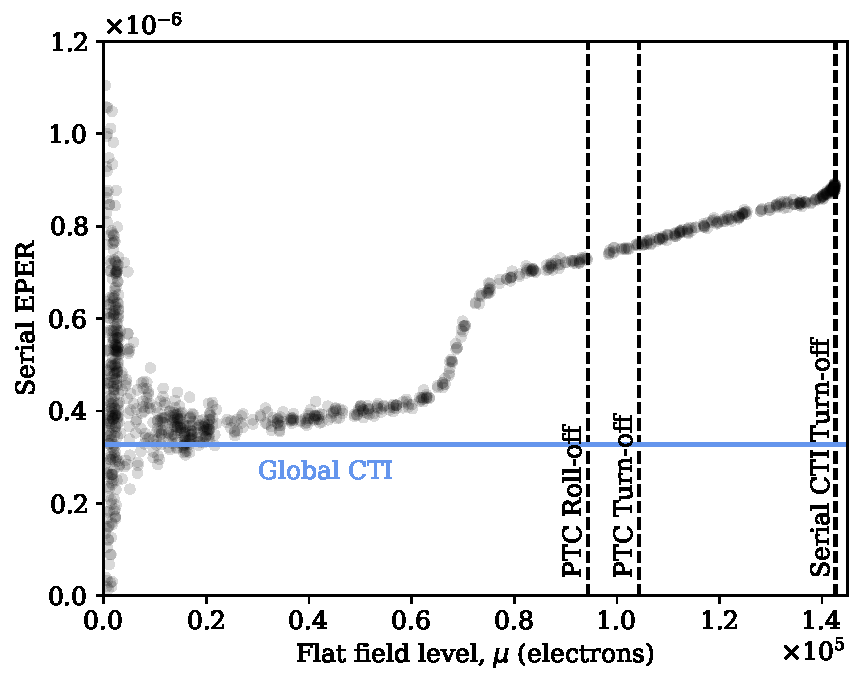
\includegraphics[width=\columnwidth]{figures/cti-det93-ampC04-serial-eper.pdf}
    \caption{Serial EPER statistics as a function of flat-field signal level for detector/amplifier R22-S10/C04.
    Vertical markers indicate the PTC rolloff and turnoff thresholds (described in \S\ref{sec:processing:calibration:ptc}) and the serial CTI turnoff derived from the low-signal trend.
    The global CTI fit produces the overall offset of the measured curve at all signal levels.}
    \label{fig:cti-serial-eper}
\end{figure}

The CTI solver simulates charge readout and each of the three effects at the amplifier image level for a given set of parameters.
The model in the simulation is parameterized by a global serial CTI parameter $b$ that is a fractional charge loss per pixel transfer, a local electronic offset described by drift scale $A_L$ and decay time $\tau_L$, and a spline-based serial charge-trap decay model whose size is allowed to depend on the signal in the last imaging column.
We perform a least squares fit that finds the optimal set of parameters that can reproduce the measured overscan statistics trend as a function of signal level.
Then the solver fits these parameters to the overscan image in stages.
First, it varies only the local offset parameters, then the global CTI parameter, and then the trap capture curve from residuals between model and data.
Exposures above configured flux limits are excluded from each stage (typically $10^4$~electrons for the global CTI fit and $1.5\times10^5$~electrons for trap fitting).

The LSST Science Requirements Document requires that total deferred charge measured by EPER be kept under a total of $5\times10^{-6}$ for signal levels below saturation level on each amplifier (citation needed).
Within the population of amplifiers in active science detectors, only 95 amplifiers do not meet this requirement without ISR correction.\todo{Express this as a fraction of the total amplifier population (95 out of how many?) and by how much those amplifiers exceed the requirement, rather than a bare count; also reconcile this number with the 26 quoted in the next sentence, since it is unclear whether they are subsets of the same population.}
Figure~\ref{fig:cti-global-histogram} shows the distribution of inferred global CTI across all amplifiers on the LSSTCam focal plane, and we show that 26 have a global CTI offset that is already above the maximum allowed threshold.
The majority of these (19) are bad amplifiers that are in the detector corners (C00, C07, C10, C17) positioned near the serial register, and it is possible that what is inferred as global CTI could be a serial trap that turns on at very low signal levels (below the $10^4$ electron level) and appears as an overall offset that is mistaken for global CTI.\todo{Support this hypothesis quantitatively: the trap size that would be needed to mimic the observed offsets, or the measured EPER behaviour of these corner amplifiers below $10^4$\,electrons.}

\begin{figure}[t]
    \centering
    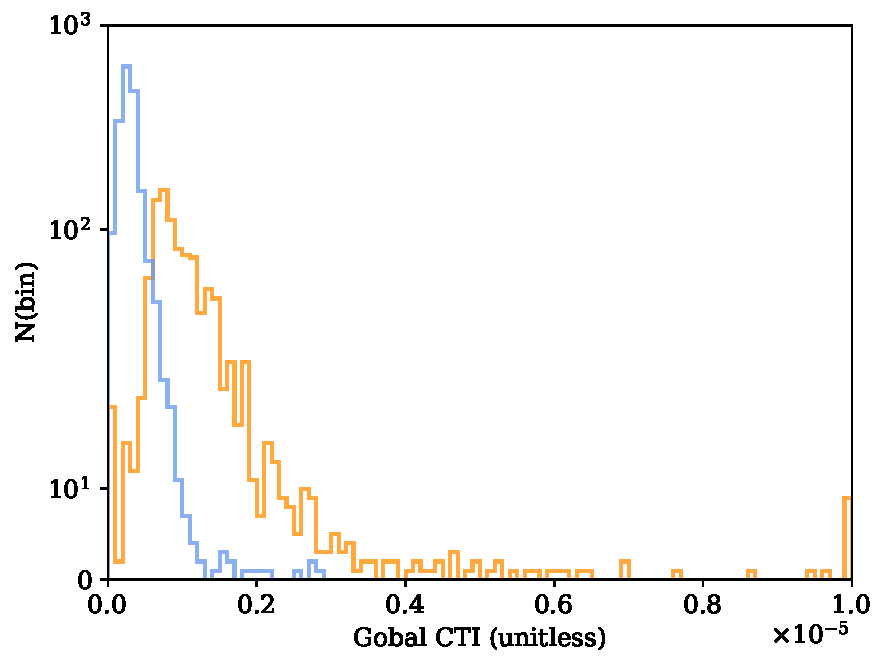
\includegraphics[width=\columnwidth]{figures/cti-det93-ampC04-global-cti-histogram.pdf}
    \caption{Distribution of inferred global serial CTI across all science sensor amplifiers on the LSSTCam focal plane.
    \textit{Blue}---Teledyne e2v (E2V) detectors; \textit{Orange}---Imaging Technology Laboratory (ITL) detectors.
    The fit to the deferred charge model allows global CTI to vary up to $1.0 \times 10^{-5}$.}
    \label{fig:cti-global-histogram}
\end{figure}
% TODO: Add CTI-corrected versions of Figure~\ref{fig:cti-global-histogram}.

When correcting deferred charge from an image during ISR, the deferred-charge correction takes in these fit parameters and applies the inverse operators from the model.
The global CTI and local-offset fits, and the inverse correction operators applied during ISR, are the same for both ITL and E2V sensors, but serial traps are fitted only on ITL since it was observed that E2V sensors had small trap size that was difficult to measure beyond noise fluctuations and already negligible enough not to require correction.\todo{Give the upper limit on E2V trap size (in electrons) and the measurement noise floor, so ``negligible'' is a stated bound rather than a judgement; likewise give the typical ITL trap size for contrast.}
After applying a deferred charge correction, we can re-compute the EPER statistics on the corrected dataset and find that all amplifiers meet the science requirements.\todo{Report the post-correction residual deferred charge (median and worst-case) against the $5\times10^{-6}$ requirement --- ``all amplifiers meet'' is much stronger with the margin attached.}

While there can be deferred charge from a charge transfer in the parallel direction (shift row-to-row), in principle this is a difficult quantity to estimate accurately from parallel overscan statistics.
EPER statistics computed in the parallel overscan region are noisy and reveal no statistically significant charge residuals, so we do not apply any parallel deferred charge correction to science images.\todo{Quote the upper limit this non-detection places on parallel CTI (value and confidence level) and compare it to the requirement, instead of only stating that nothing was significant.}

% During science ISR, this product is applied at the deferred-charge correction step in Figure~\ref{fig:isr-pipeline}; see \S\ref{sec:isr-science}.


\subsection{Photon Transfer Curve (PTC)} \label{sec:processing:calibration:ptc}

The photon transfer curve (PTC) characterizes how pixels respond to varying signal levels in a given wavelength band by measuring covariances between pixels in flat-field exposures across a range of illumination levels.
This dataset provides critical calibration information including amplifier-level read noise and gain for variance plane estimation, saturation thresholds for masking, and parameters needed to correct for non-linearity, charge transfer inefficiency (CTI), and the brighter-fatter effect.
All of these parameters can differ at the amplifier level.\todo{Quantify the amplifier-to-amplifier spread in the key PTC outputs for DP2 (gain, read noise, PTC turnoff): median and range, ideally split by vendor.}

% The photon transfer curve used to calibrate LSSTCam for DP2 is measured from $543\times2$ flat field exposures at evenly spaced illumination levels as low as 100~analog-to-digital units (ADU) and reaching at least 10\% beyond saturation.
% At each illumination level, a pair of flats was acquired by varying both LED output and exposure time to achieve the target signal.
% We measure the covariance between pixels on the difference image of the two exposures to remove variations sourced by static, fixed-pattern artifacts.

Let $F_1$ and $F_2$ denote the two flats at a given illumination level, and let $\mu = \mathrm{avg}(F_1,F_2)$ denote the mean signal level (in ADU) over the image and away from the detector edges.
The covariance between a pixel $\mathbf{x}=(0,0)$ and a neighbor at pixel $\mathbf{x}'=(i,j)$ is:
\begin{equation}
    C_{ij} \;=\; \tfrac{1}{2}\,
    \mathrm{Cov}\!\left(F_1(\mathbf{x})-F_2(\mathbf{x}),\,
                       F_1(\mathbf{x}')-F_2(\mathbf{x}')\right).
\end{equation}

% Following the standard front-illuminated CCD convention, serial (row) readout proceeds along $(1,0)$ and parallel (column) readout along $(0,1)$.

\paragraph{Pre-model fit}
Preliminarily, we fit only the variance to an approximate exponential relation derived in \citet{2019A&A...629A..36A} (their Eq.~16).
\begin{equation}
    C_{00}^{\mathrm{exp.\,approx}}(\mu) = \frac{1}{2 g^2 a_{00}}\bigl[\exp(2 a_{00} \mu g) - 1\bigr] + \frac{n_{00}}{g^2}\ .
\end{equation}
In this expression, covariances are contributed by a gain $g$ (electrons$/\mathrm{ADU}$), noise pedestal $n_{00}$ (electrons$^2$), and a single brighter-fatter coefficient $a_{00}$ ($1/$electrons) which has the effect of decreasing the image variance.

Near saturation, the variance deviates from this functional form, exhibiting a gradual rollover rather than a sharp cutoff due to electrostatic effects that are difficult to model analytically.\todo{Give typical values for $\mu_0$ and $\tau$, and the typical separation between the rolloff and turnoff levels, so ``gradual'' is quantified.}
On top of the exponential approximation, we introduce an empirical saturation term:
\begin{equation}
    C_{00}^{\mathrm{sat}}(\mu) = \left\{
        \begin{array}{ll}
            -e^{-(\mu-\mu_0)/\tau} & \mu \ge \mu_0 \\
            0 & \mu < \mu_0
        \end{array}
    \right.,
\end{equation}
where $\mu_0$ marks the onset of the PTC ``rolloff'' effects and $\tau$ controls the shape of the rollover.
The total preliminary fit model is $C_{00}^{\mathrm{prelim.}}(\mu) = C_{00}^{\mathrm{exp.\,approx}}(\mu) + C_{00}^{\mathrm{sat}}(\mu)$ to the unweighted points. This fit is performed iteratively with additional 3~sigma clipping until convergence.
The ``PTC turnoff'' is defined as the signal level of the last unmasked point following the fit to only the exponential approximation, typically corresponding to the maximum of the variance curve and generally higher than the rolloff threshold.
The ``PTC rolloff'' is the signal level where $C_{00}^{\mathrm{prelim.}}(\mu)$ and $C_{00}^{\mathrm{exp.\,approx}}$ deviate by more than 1\%.

\paragraph{Final model fit}
With the remaining points below the PTC rolloff, we fit the complete covariance expansion from \citet{2019A&A...629A..36A} (their Eq.~20):
\begin{equation}
    \begin{aligned}
    C_{ij}^{\mathrm{model}}(\mu) = \frac{\mu}{g} \Bigl[ \delta_{i0}\delta_{j0}
      &+ a_{ij}\mu g \\
      &+ \frac{2}{3}\left([\mathbf{a}\otimes\mathbf{a} + \mathbf{ab}]_{ij}\right)(\mu g)^{2} \\
      &+ \frac{1}{6}\left(2\mathbf{a}\otimes\mathbf{a}\otimes\mathbf{a} + 5\mathbf{a}\otimes\mathbf{ab}\right)_{ij}(\mu g)^{3} \\
      &+ \mathcal{O}[(\mu g)^4]
    \Bigr] + \frac{n_{ij}}{g^2},
    \end{aligned}
    \label{eq:cov_model}
\end{equation}
where $a_{ij}$ (electrons)$^{-1}$ represents the fractional change in pixel area per stored charge due to boundary motion from the brighter-fatter effect, $b_{ij}$ (electrons)$^{-1}$ captures weaker time-dependent corrections, $g$ is the gain (electrons$/\mathrm{ADU}$), and $n_{ij}$ is the constant noise contribution (electrons)$^2$ (e.g., $n_{00}\sim (5.7\,\mathrm{electrons})^{2}$ on the diagonal, with off-diagonal terms determined by read electronics and overscan).
The symbol $\mathbf{ab}$ denotes element-wise matrix multiplication, and $\otimes$ represents discrete convolution.
In practice, the $b_{ij}$ parameter is inferred to be just noise around a value of zero.\todo{State the constraint: the measured $b_{ij}$ scatter and the corresponding upper limit, and the size of $b_{ij}$ relative to $a_{ij}$ that would matter for the correction.} The size of the covariance matrix ($n \times n$) is determined by the range of the brighter-fatter effect (see \S\ref{sec:processing:calibration:bf}).
Figure~\ref{fig:ptc-fit-example} shows an example fit for amplifier~C03 on detector~94, illustrating the measured $C_{00}$ points, the preliminary exponential approximation with saturation roll-off, and the final variance from Eq.~\ref{eq:cov_model}.

\begin{figure*}[t]
    \centering
    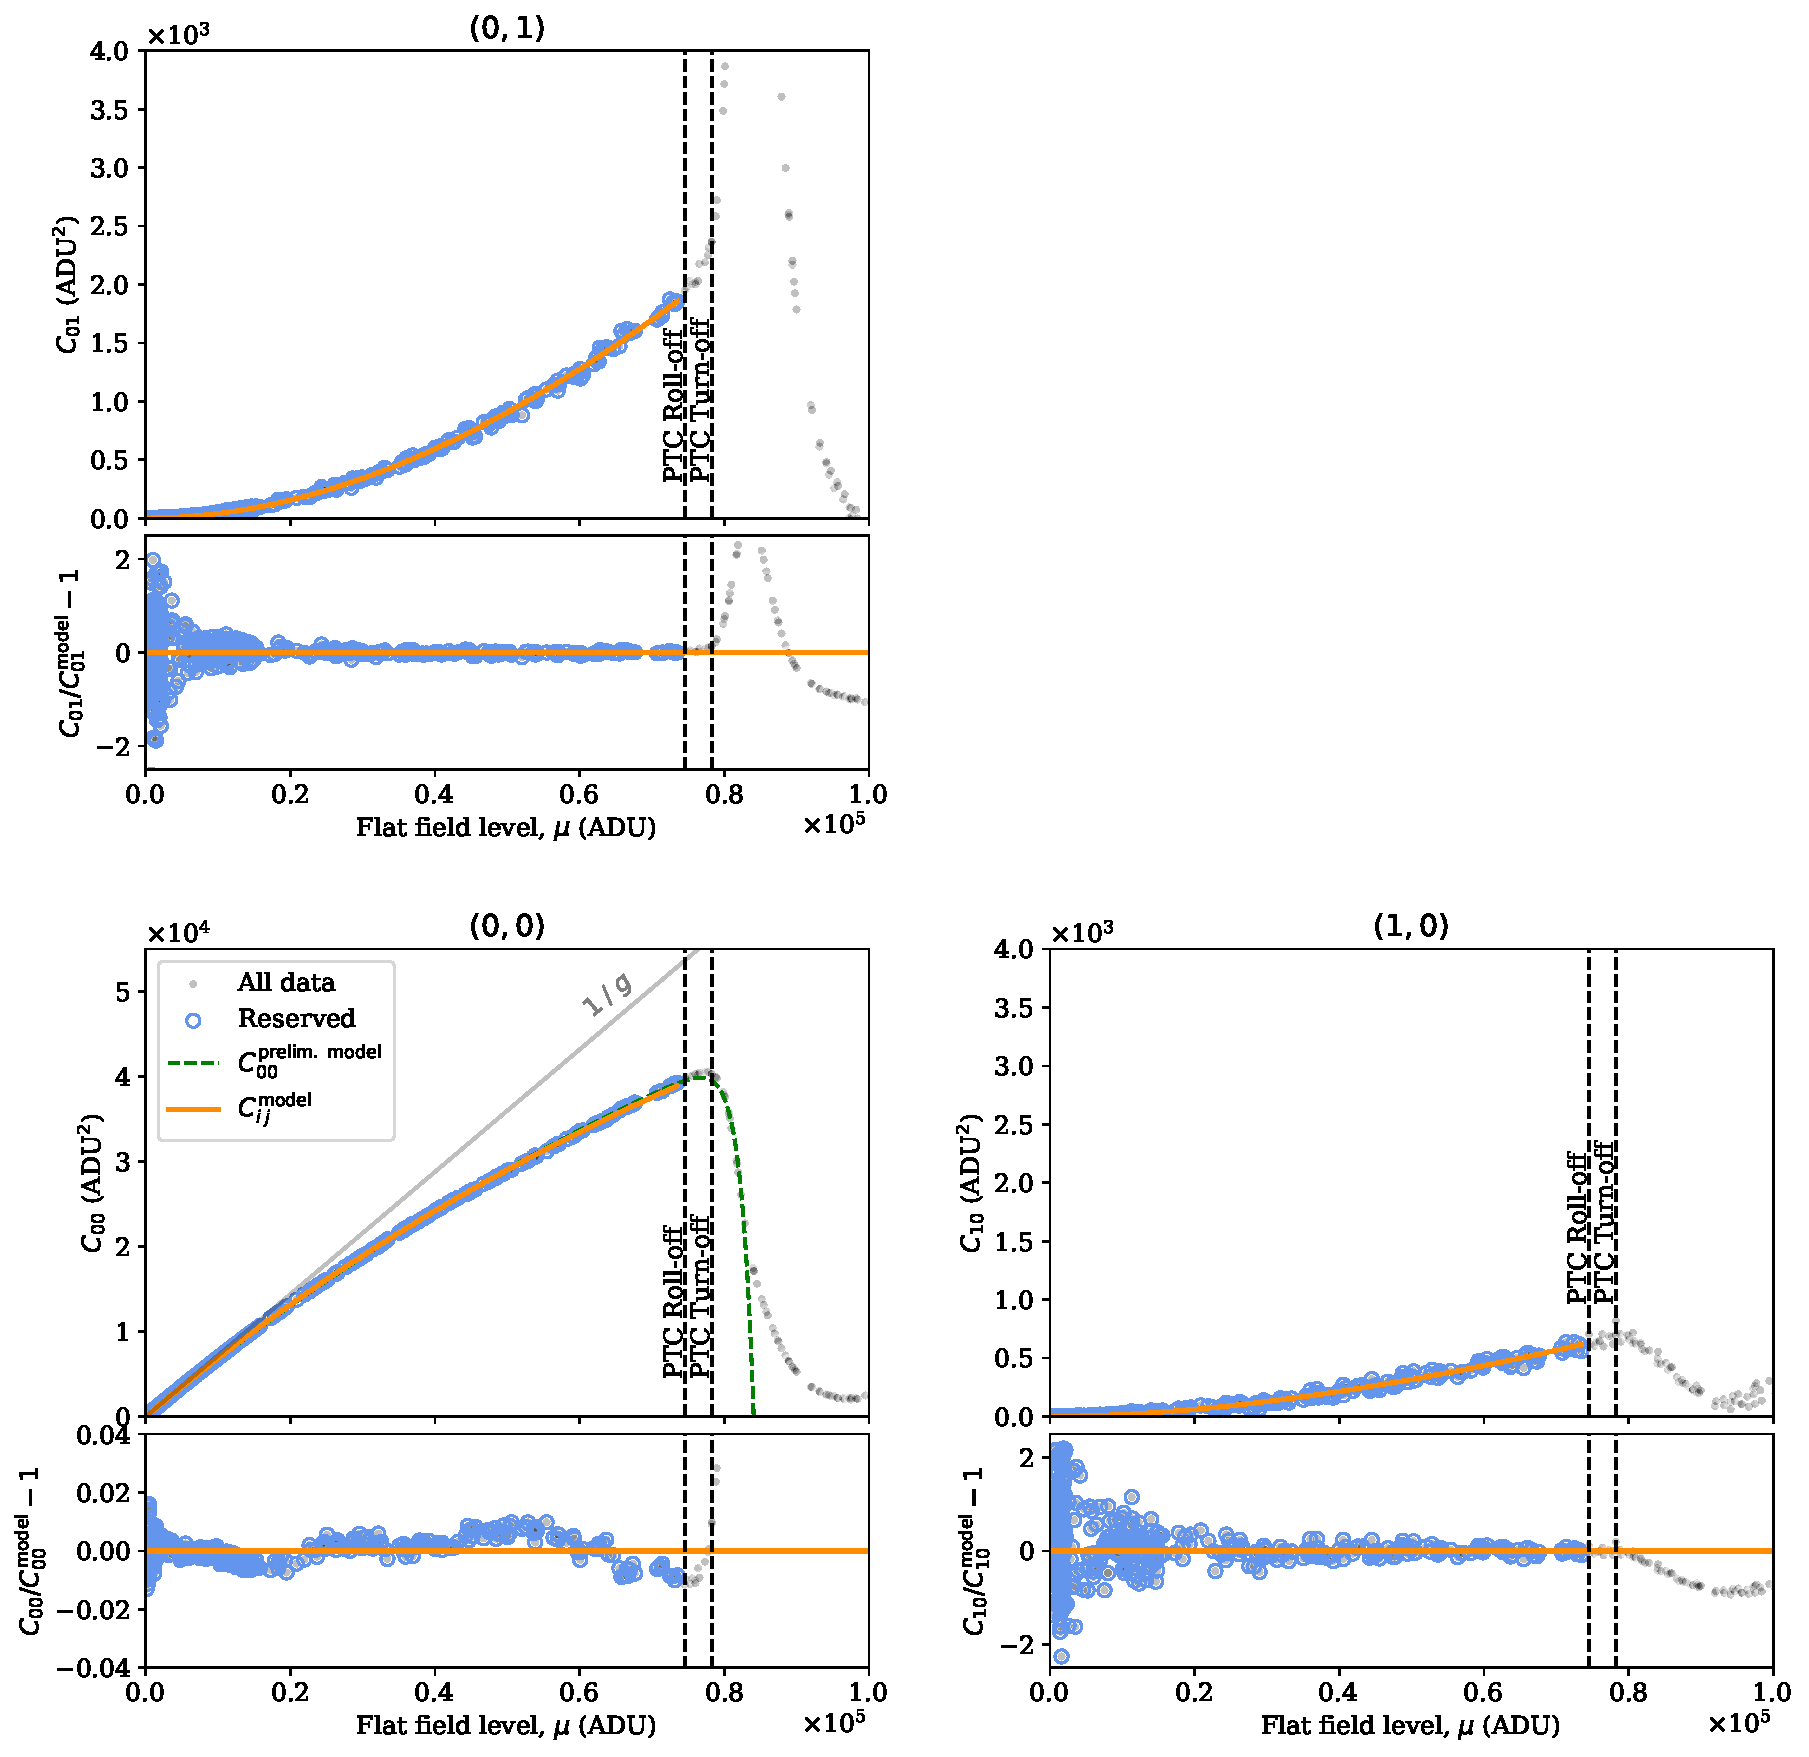
\includegraphics[width=\textwidth]{figures/ptc-triangle-det94-ampC03.pdf}
    \caption{Example PTC fit for amplifier~C03 on LSSTCam detector~94.
    Measured $C_{00}$ covariance points are compared to the preliminary fit (exponential approximation plus saturation roll-off) and the final full-covariance model variance.
    Vertical markers indicate the PTC rolloff and turnoff thresholds.}
    \label{fig:ptc-fit-example}
\end{figure*}

Because the gains are fit independently per amplifier, small fitting residuals can leave flux discontinuities at amplifier boundaries within a detector.\todo{Quantify the discontinuity before adjustment (percent flux step across an amplifier boundary) and the statistical uncertainty on the per-amplifier gain fit that produces it.}
We add a subsequent step that measures the relative offsets between amplifiers in flat fields after gain correction and computes small adjustments to the gain to make the detector image continuous while preserving the average gain across the detector.
We compute the average gain adjustment in flat fields across a range of signal levels, and use these to produce overall ``adjusted gains''.
The adjustments to the gain are always small (less than 0.03), and uncorrelated between detectors.\todo{Clarify the units of the 0.03 (electrons/ADU or fractional?) and give the distribution --- median and 95th percentile --- rather than only a bound; also quantify ``uncorrelated'' with a correlation coefficient if that claim is load-bearing.}
These final gains are used for conversion of science images to electron units and construction of the variance plane for source detection.

The PTC calibration products are applied during instrument signal removal of science images in three ways.
First, the gain converts pixel values from ADU to electrons.
Second, the gain and read noise inform variance plane estimation.
Third, the saturated pixel mask flag (denoted ``SAT'') is set for all pixels with values greater than or equal to the PTC turnoff threshold.

% During science ISR, PTC-derived gains, variance-plane inputs, and saturation masking are applied at the steps shown in Figure~\ref{fig:isr-pipeline}; see \S\ref{sec:isr-science}.


\subsection{Brighter-Fatter Effect (BFE)} \label{sec:processing:calibration:bf}

The brighter-fatter effect (BFE) is the first influence the detector has on an incident signal (Figure~\ref{fig:detector-boxes}).
Accumulated electrons in a pixel repel incoming charges into neighboring pixels.
Brighter point sources therefore appear wider in the recorded images.
This electrostatic effect reduces to an effective change in pixel area and introduces correlations between nearby pixel values.
The effect is intrinsic to thick CCDs and can significantly bias point-spread-function (PSF) photometry and shape measurement.\todo{Quantify ``significantly'': the uncorrected PSF size growth with source flux (e.g.\ percent change in second moments per decade of flux) and the resulting photometric/shape bias, relative to the LSST requirement.}

The BFE has been extensively characterized for LSSTCam by laboratory and in-dome commissioning measurements \citep{2024PASP..136d5003B}.
The strength of the effect is anisotropic ($a_{01}/a_{10} \sim 3$), long-ranged ($\sim 10$~px), and wavelength dependent.
It is also about twice as strong in the E2V-family detectors as in ITL-family detectors.

Several BFE correction methods have been proposed and implemented in the LSST Science Pipelines \citep{2015JInst..10C5032G,2018AJ....155..258C,2023A&A...670A.118A,2024PASP..136d5003B}, and they differ widely in their underlying assumptions.
\citet{2024PASP..136d5003B} found that modeling individual boundary shifts for every pixel (N, S, E, W) is required for adequate correction at the level needed for LSST Y10 science requirements.
Flat-field pixel correlations can measure only the net per-pixel area change, so determining these boundary shifts requires additional electrostatic modeling.
For processing raw images from DP2, we use the \citet{2023A&A...670A.118A} algorithm developed for Hyper Suprime-Cam, which derives from electrostatic physics and treats each pixel boundary individually.

% The correction assumes three simplifying conditions.
% First, the average charge current into a pixel is approximately constant during a long exposure, even when the PSF varies with time.
% Second, fourth-order terms in Eq.~\ref{eq:cov_model} are negligible; at the scale of the BFE, the corresponding coefficients are of order $10^{-24}$.
% Third, photons convert to electrons quickly after entering the detector.
% Simulations and empirical modeling indicate that most photons in $u$ through $i$ bands convert within the top few microns of silicon, while the BFE influence on charge drifting to the pixel bottom occurs primarily in the last several microns.
% Chromatic effects are therefore likely negligible for photons with wavelengths across the LSST bandpasses.

\begin{deluxetable}{ll}[t!]
    \tablecaption{Parameter Priors for the Electrostatic BFE Model Fit\label{tab:bf-electrostatic-fit-priors}}
    \tablehead{
        \colhead{Parameter} & \colhead{Prior}
    }
    \startdata
        Si thickness, $t$ ($\mu$m)        & $100$ (fixed) \\
        Pixel size, $p$ ($\mu$m)         & $10$ (fixed) \\
        Charge cloud height, $z_q$ ($\mu$m)      & $0 \leq z_q \leq t/2$ \\
        Charge cloud length, $a$ ($\mu$m)        & $10^{-5} \leq a \leq 0.35\,p$ \\
        Charge cloud width, $b$ ($\mu$m)         & $10^{-5} \leq b \leq 0.35\,p$ \\
        Potential well vertex height,\\horizontal $z_{sh}$ ($\mu$m)    & $0 \leq z_{sh} \leq t/2$ \\
        Potential well vertex height,\\vertical $z_{sv}$ ($\mu$m)    & $0 \leq z_{sv} \leq t/2$ \\
    \enddata
    \tablecomments{Priors on the fit parameters are informed by pixel-level simulations of the electric fields in these pixels \citep{2017JInst..12C3091L}. The potential well vertices refer to the heights above the front-side of the CCD to the saddlepoints in the electric field that defines the pixel boundaries in the vertical (0, 1) and horizontal (1, 0) directions. The electrostatic model assumes that the stored charge cloud in the sensor takes the form of a flat, rectangular sheet of charge with length ($a$) and width ($b$). The inequality constraints $z_{sh} > z_q$, $z_{sv} > z_q$ are enforced during optimization, which is true in the unsaturated signal level regime.}
\end{deluxetable}

Calibration of the BFE using this algorithm takes the form of modeling a charge cloud at the bottom of a pixel, computing
how the effective areas of nearby pixels would be expected to change electrostatically in response. It adjusts some geometric parameters (summarized in Table~\ref{tab:bf-electrostatic-fit-priors}), and solves
Gauss's law to compute the shift of pixel boundaries and the relative change in pixel area from each shift ($\mathbf{a}^{\mathrm{N}}$,
$\mathbf{a}^{\mathrm{S}}$, $\mathbf{a}^{\mathrm{E}}$, $\mathbf{a}^{\mathrm{W}}$).
We optimize these parameters to best fit the
measured net pixel area changes ($\mathbf{a}$ from Eq.~\ref{eq:cov_model}):
\begin{equation}
    \mathbf{a} = \mathbf{a}^{\mathrm{N}} + \mathbf{a}^{\mathrm{S}} + \mathbf{a}^{\mathrm{E}} + \mathbf{a}^{\mathrm{W}}.
\end{equation}

In principle, the BFE can vary amplifier-to-amplifier, but we have observed only noise-level variations in the pixel distortion matrices across amplifiers and even detector families.\todo{Give the amplifier-to-amplifier scatter in $a_{01}$/$a_{10}$ against the per-amplifier measurement uncertainty, which is the quantitative basis for fitting at the detector level; note this also appears to sit in tension with the statement above that the effect is twice as strong in E2V as in ITL.}
For this reason, and to avoid discontinuous amplifier boundaries, the fit is performed at the detector level.
All $a_{ij}$ matrices from well-behaved amplifiers are 3$\sigma$-clipped elementwise and averaged into a detector-mean $a_{ij}$; the scatter becomes the per-element uncertainty, and a single fit is run against this average pixel distortion matrix.
The output calibration data product is the set of model parameters and a model that can be evaluated per-detector.

Applying this calibration to remove the effect during ISR uses the boundary-shift matrices $\mathbf{a}^{\mathrm{N}}$, $\mathbf{a}^{\mathrm{S}}$, $\mathbf{a}^{\mathrm{E}}$, and $\mathbf{a}^{\mathrm{W}}$ to redistribute flux accordingly.
We tile these into two, $(2n+1)\times(2n+1)$, convolution kernels $K^{H}$ and $K^{V}$ for the horizontal and vertical shifts, respectively; we apply sign flips and edge adjustments so each matrix sums to zero.
These matrices need not be symmetric, which is more realistic per \citet{2024PASP..136d5003B}.
Figure~\ref{fig:ebf-kernels} shows an example pair of these kernels for amplifier~C03 on detector~94, illustrating the dipole-like, charge-conserving structure that redistributes flux across the vertical and horizontal pixel boundaries.

\begin{figure}[t]
    \centering
    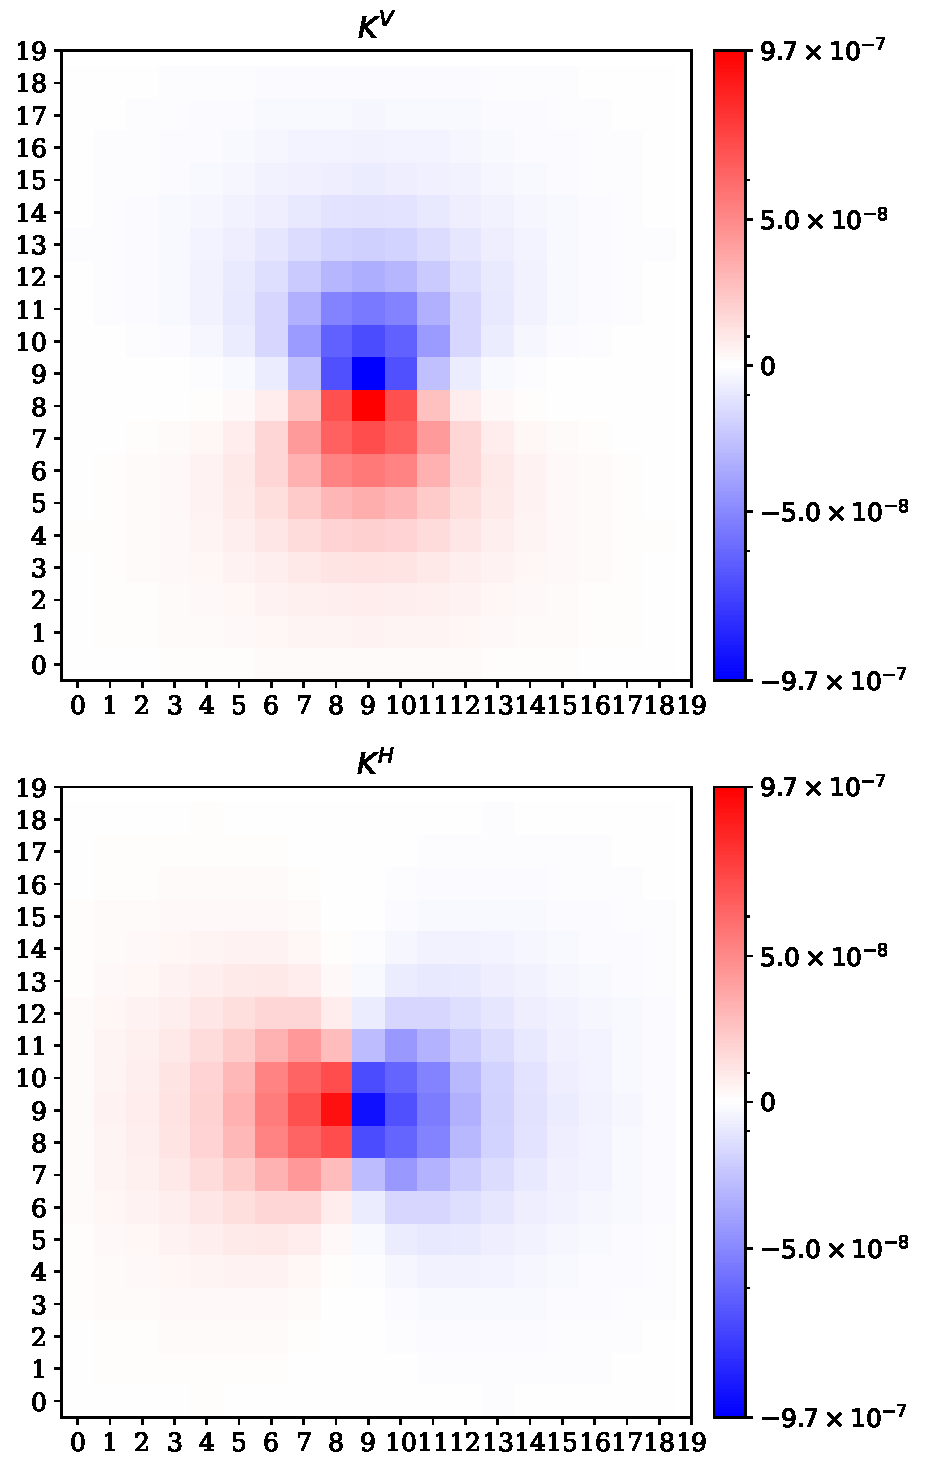
\includegraphics[width=\columnwidth]{figures/ebf-det94-ampC03-kVH.pdf}
    \caption{Example BFE correction kernels $K^{V}$ (vertical) and $K^{H}$ (horizontal) derived from the electrostatic BFE model for amplifier~C03 on LSSTCam detector~94.
    The diverging color scale shows the fractional charge redistributed across pixel boundaries; each kernel sums to zero to conserve charge and exhibits the antisymmetric dipole structure that moves flux from the brighter pixel to its neighbors.}
    \label{fig:ebf-kernels}
\end{figure}
For an image $Q_{ij}$ in natural gain-corrected units of electrons, the amount of charge lost over the vertical and horizontal boundaries is:
\begin{align}
    \delta^{H}_{ij} &= \tfrac{1}{2}\!\!\sum_{kl}\!\!K^{H}_{kl}\,Q_{i-k,\,j-l}, \notag \\
    \delta^{V}_{ij} &= \tfrac{1}{2}\!\!\sum_{kl}\!\!K^{V}_{kl}\,Q_{i-k,\,j-l},
    \label{eq:bf-shift}
\end{align}
The $1/2$ prefactor accounts for the average BFE assuming a constant rate of charge accumulation during an exposure.
The corrected image is assembled by removing the charge each pixel lost across its $N$/$E$ boundaries and adding what it gained from $S$/$W$ neighbors, guaranteeing charge conservation by construction, $\sum_{ij}Q^{\mathrm{corr}}_{ij}=\sum_{ij}Q_{ij}$.
This correction does not require iterative convolutions. Unlike the \citet{2018AJ....155..258C} algorithm used for DP1 \citep{2026AJ....171..360V}, which requires multiple convolutions to reach convergence, we perform exactly two convolutions with the horizontal and vertical boundary-shift matrices.\todo{Quantify the gain from this: the typical number of iterations the DP1 algorithm required, and the resulting speedup in per-detector ISR wall-clock time --- and, if available, whether correction quality changed.}

% During science ISR, the BFE correction is applied at the step shown in Figure~\ref{fig:isr-pipeline}; see \S\ref{sec:isr-science}.


\subsection{Combined Bias} \label{sec:processing:calibration:bias}

A bias image is a zero-second exposure read out with the shutter closed, and so records the electronic pedestal of the readout chain in the absence of any accumulated charge.
Overscan correction removes the component of that pedestal that varies from exposure to exposure, while the combined bias measures the static two-dimensional electronic structure that remains and is subtracted from every science image.

To remove this remnant signal that is not already removed by the previous calibrations, a combined bias frame is subtracted from the exposure.
This combined bias is constructed from the per-pixel clipped mean of a large number of input zero-second bias frames.\todo{Quantify the residual static structure the combined bias removes: its peak-to-peak and RMS amplitude in electrons, so the reader knows the size of the signal being corrected.}
These input bias frames have all of the corrections discussed up until this point applied.
For LSSTCam, these combined biases have 400 input exposures, which reduces the noise in the correction.\todo{State the resulting noise: with 400 frames the combined-bias noise is read noise$/\sqrt{400}$ --- give that value in electrons and compare it to the single-frame read noise, so the choice of 400 is justified numerically.}
CZW: quick study to see if we have any with fewer than 400 exposures.

\subsection{Combined Dark} \label{sec:processing:calibration:dark}

A dark image is an exposure taken with the shutter closed, and measures the signal that accumulates in proportion to integration time rather than to incident light. It is dominated by absorption from thermally generated infrared photons, called dark current, together with any glow from the readout electronics.\todo{Give the measured dark current level (electrons/pixel/s, median and range across the focal plane) and the amplitude of the readout glow, plus how much signal that amounts to in a 30\,s science exposure.}
These artifacts are removed by scaling the dark to the exposure time of the science image and subtracting it.

Similar to the bias, we construct a combined dark frame from a large number of 30-second exposures, with that time chosen to match the standard exposure time of a science exposure.
As before, all of the previous calibrations are applied to these dark frames, including the bias correction.
These exposures have an additional cosmic ray rejection step applied after the ISR processing, as these longer exposures may have more of these features than are found on the bias frames.\todo{Quantify the cosmic-ray rate (events or affected pixels per detector per 30\,s exposure) and the fraction of pixels rejected, instead of ``may have more''.}
The combined dark is again created from the per-pixel clipped mean, and for LSSTCam we have a target of 400 input frames.
CZW: I know we don't always hit that, put words here.

\subsection{Combined Flats} \label{sec:processing:calibration:flats}

A flat field measures the relative response of the system to uniform illumination, capturing both pixel-to-pixel variations in quantum efficiency and larger-scale structure imposed by the optics, the filter transmission, and vignetting of the focal plane.
Dividing a science exposure by the combined flat normalizes this response, so that a source of a given flux produces the same measured signal regardless of where it lands on the focal plane.

Although flat-field images are a common astronomical correction, the large field-of-view of LSSTCam makes generating this calibration a particular challenge.
In addition to ensuring consistent illumination across this field-of-view, there is an added complication that the ITL and E2V detectors have different responses as a function of wavelength.\todo{Quantify the ITL/E2V response difference (the fitted ratio per band, which the six-node spline pass already measures) rather than only noting that it exists.}
One final complication comes from the finite choices of LEDs in the flat-field illumination system described in Section \ref{sec:data:calsys:flat_field_illuminator}.
We anticipate that we will be able to construct higher quality synthetic flats from sequences of laser-illuminated monochromatic flats in the future, for DP2 we have chosen to construct ``anaglyph'' flats for most bands.\todo{Quantify what the two-LED anaglyph approximation costs relative to a true synthetic flat: the residual chromatic error expected (in mmag across the focal plane), which is what ``higher quality'' should mean here.}

These anaglyph flats superimpose a red-side and a blue-side flat to construct a single flat across a full LSST bandpass. For a given filter, we combine a pair of flat-field images that have each been observed with a single active LED illuminating the flat-field screen.
For the subsequent discussion, these two sets of input flat-field images are referred to as the ``red'' and ``blue'' exposures, depending on the wavelength of the two LEDs within the filter bandpass that final flat field will be used for.
These anaglyph flats have been constructed for each of the $grizy$ filters.
This process is unavailable for the $u$ filter since a sufficiently blue ultraviolet LED was not available, nor was there space to fit one inside the projection system, and so flats for this filter are constructed from only a single set of flats (with an LED that is at the red end of the bandpass).
A bluer ultraviolet LED will be available to be periodically swapped in and out for DP1 calibrations.

To begin the construction of new flats, the input exposures are processed through the ISR steps that are applied prior to flat correction, including the bias, dark, crosstalk, gain application, linearization, CTI, and overscan (CZW: reorder to be in order).
Statistics are measured on these processed exposures, determining the median value and dispersion on each detector.
Normalization factors are then measured for the red and blue inputs separately based on these statistics, which should account for any differences in the absolute flux received in each exposure over all detectors.
These normalization factors are used to properly scale the inputs before they are combined using a clipped mean per pixel into separate intermediate red and blue flats.

These intermediate flats include gradients related both to how well the flat-field illumination and screen were oriented and due to the vignetting of the focal plane itself.\todo{Give the amplitude of each gradient separately (percent across the focal plane for the planar illumination gradient, and the vignetting depth at the outer radius), so the reader can see which dominates.}
Both types of gradients are measured next, so that contribution can be removed from the final flat.
An initial six-node radial spline model is fit to the full binned focal plane image of the intermediate flats.
This initial model is used to constrain both the centroid of the focal plane and the observed ratio of the ITL to E2V detectors, to account for their possibly different response.
These parameters are then used for a 15-node radial spline model that is more careful about fitting the observed vignetting at high focal plane radii.\todo{Quantify what the 15-node model buys over the 6-node one (residual RMS for each), and state the radius beyond which vignetting becomes significant.}
This second fit uses a fixed ITL/E2V ratio measured during the first pass, to reduce the degrees of freedom in the final fit.
An additional planar gradient is also included in this second fit, to account for simple illumination differences.

The measured gradients are then removed from the intermediate flats.
The planar gradients are simply divided from the per-detector intermediate flats.
The radial gradient is scaled by a reference gradient to reduce the effects of the vignetting, and to match the vignetting observed in on-sky data (CZW: I need to explain reference gradient better).\todo{State how well the flat-derived and on-sky vignetting agree after this scaling (residual percent as a function of focal-plane radius) --- this is the key quantitative test of the flats.}
A final normalization factor is applied to scale the entire flat to match the intensity level observed within the central 25mm of the focal plane.
With these gradient-corrected intermediate flats generated, a final flat is constructed by combining the red and blue intermediates with a filter-specific mixture weight, as listed in Table \ref{tab:anaglyph_ratios}.

\begin{table}[]
  \begin{tabular}{lll}
    Band & Blue weight & Red weight \\
    $g$ & 0.63 & 0.37 \\
    $r$ & 0.50 & 0.50 \\
    $i$ & 0.476 & 0.524 \\
    $z$ & 0.65 & 0.35 \\
    $y$ & 0.52 & 0.48 \\
  \end{tabular}
  % TODO(ref): \label comes before \caption, so \ref{tab:anaglyph_ratios} resolves to the section number (5.11 in the .aux) instead of the table number; move the \label after the \caption.
  \label{tab:anaglyph_ratios}
  \caption{Mixture weights for anaglyph flat construction.\todo{Say how these weights were derived (matching the LED-weighted effective wavelength to the band's effective wavelength?) and give the uncertainty on each weight plus the sensitivity of the resulting flat to a weight error.}}
\end{table}
